\documentclass[12pt]{article}
\usepackage[margin=1in]{geometry} % change margins
\usepackage{graphicx} % inserting images
\usepackage{caption} % captions
\usepackage{amsmath} % for better math
\usepackage{verbatim} %used for comment blocks
\usepackage{mathtools}
\usepackage[english]{babel}
\usepackage[colorinlistoftodos]{todonotes}
\usepackage{placeins}
\usepackage[square, sort, numbers]{natbib}
\usepackage{url}
\usepackage{setspace}
\usepackage{breqn}
\usepackage{subcaption}
\usepackage{textcomp}
\usepackage{float}
\usepackage{leftidx}
\usepackage{bm}
\usepackage[titletoc,toc, title]{appendix}
\usepackage[utf8]{inputenc}
\usepackage{diagbox}
\usepackage{hyperref}
\usepackage{tcolorbox}

\usepackage{amsmath,amssymb,braket,cancel,nicefrac,physics,tensor,slashed}
\usepackage{color,empheq,enumitem,forloop,graphicx,microtype,subcaption,verbatim,wrapfig,pdfpages,titlesec}
\usepackage{array,booktabs,multicol,multirow,tabularx} 

\usepackage{fancyhdr}
\addto\captionsenglish{\renewcommand{\chaptername}{Lab}}

\def\cesar#1{{\color{blue}[#1]}}
\def\anhkhoi#1{{\color{olive}[#1]}}
\def\nik#1{{\color{red} [#1]}}

\tcbset{colback=blue!5!white,colframe=blue!75!black,center,halign=justify,width=0.9\textwidth,fonttitle=\bfseries}

\linespread{1.15}
\title{Tutorial: Data Analysis Practice}
\author{Nikolas Provatas, Anh-Khoi Trinh, Cesar Daniel Rodriguez Rosenblueth}
\date{}

\begin{document}

\maketitle

\section{Learning objectives}
\begin{itemize}
\item Learn how to use Excel.
\item Compute certain basic mathematical statistics.
\item Introduction to data analysis.
\end{itemize}

\section{Introduction}
This lab will be an interactive demo lab where teaching Assistants will help you  learn how to use Excel and to apply it to the concepts presented in the \textbf{Data analysis} chapter. We recommend that you read the \textbf{Data Analysis} and familiarize yourself to Excel before attending this session. The first part is a mandatory tutorial session and will be scheduled in the Lab information document on MyCourses.

\section{In-class tutorial}
During the in-class tutorial session, you will familiarize yourself with Excel. You will be guided through this exercise by the TAs.

\begin{itemize}
\item Open the Excel document found at \anhkhoi{location}.
\item Explore the user interface. Note that data is best presented in columns.
\item Learn how to organize your spreadsheet: resize, split and merge cells.
\item In a adjacent column, calculate the resistance $R$. 
\item Calculate the sum of resistances $R$ by using  \verb|=SUM(x)|.
\item Calculate the average resistance $\bar{R}$ in two ways: by using the integrated function  \verb|=AVERAGE(x)| and by dividing the sum that you calculated previously by the total number of cells.
\item For each value of resistance $R_i$, calculate the difference
\begin{equation}
R_i - \bar{R},
\end{equation}
in a separate column by ``dragging" the first cell downwards.

\item Calculated the square of the difference calculated above in another column.
\item In two other columns, calculate the standard deviation by using \anhkhoi{eq.~\eqref{YY}} of the lab manual with the values that you calculated previously, and by using the function \verb|=STDEV.P(x)|. 
\end{itemize}

\noindent Now we will learn how to plot data, and how to obtain a linear regression.
\begin{itemize}
\item Select the columns of $I$ and $V$, perform a scatter plot.
\item Put in manual error bars.
\item Display a linear trendline with the fit equation and its $R^2$ value. The fit coefficient is your ``fit resistance" $R_{fit}$.
\end{itemize}

%\noindent Now we will compare this fit equation to our data. 
%\begin{itemize}
%\item To start, copy the $I$ column to another area of your spreadsheet.
%\item In the column next to it, write the fit equation such that this will be your ``Fit $V$" column.
%\item Plot $V$ vs $I$, and ``Fit $V$" vs $I$ on the same graph. Add error bars only on the $V$ vs $I$ dataset and compare the two graphs qualitatively.
%\end{itemize}

\noindent Let us now compare the resistance from the data, the average and the fit.
\begin{itemize}
\item On another area of your spreadsheet, write a column with the current values $I$. 
\item In an adjacent column, rewrite the resistance $R_i$ calculated previously with its corresponding standard deviation.
\item In another column, write the average resistance $\bar{R}$ for all values of $I$.
\item Add a column of the fit resistance $R_{fit}$ for all values of $I$.
\item Plot $R$ vs $I$ for all three datasets: the measurement $R_i$, the mean $\bar{R}$ and the fit $R_{fit}$. Note that $\bar{R}$ and $R_{fit}$ should be horizontal constants. Compare them.
\end{itemize}

\section{Homework Exercise}
As homework, you will analyse a given dataset. Consider a setup where you can measure the electric force between two charges as shown in Fig.~\ref{Fig:lab0-session2-setup}. 
\begin{figure}[h]
\centering
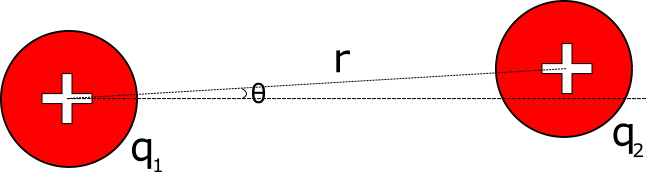
\includegraphics[width=0.8\textwidth]{lab0-session2}
\caption{Setup for the data of Session 2. Two charges $q_1$ and $q_2$ are separated by a distance $r$, and at an angle $\theta$ with respect to some axis horizontal to $q_1$.}
\label{Fig:lab0-session2-setup}
\end{figure}

Given this dataset, you must find how the electric force on $q_1$ is affected by the following parameters:
\begin{itemize}
\item Charges $q_1$ and $q_2$.
\item The angle $\theta$ with respect to a horizontal axis separating $q_1$ from $q_2$.
\item Distance $r$ between the charges.
\end{itemize}
For each dataset, the variables that are held constant are summarized in Table~\ref{Tab:constants}. 

Let us denote one of the varying parameters above as $x$. The force $f$ will be a function of $x$ such as $f(x)$. In the data file, the four columns are separated as shown below.
\begin{table}[h]
\centering
\begin{tabular}{c c c c}
$x$, & $\sigma_x$, & $f(x)$, & $\sigma_f$
\end{tabular}
\end{table}
The columns are separated by commas. This is called a CSV file.
You are to plot the data and perform different fits to verify the $R^2$ value and how the fits compare to the error bars.
You should explore other fits than just the linear one.

\begin{table}[h]
\centering
\begin{tabular}{c|c}
file name & constant parameters \\ \hline
varying-q1 & $q_2=100$, $\theta=0$, $r=10^{-9}$ \\
varying-q2 & $q_1=100$, $\theta=0$, $r=10^{-9}$ \\
varying-theta & $q_1=400$, $q_2=400$, $r=10^{-9}$ \\
varying-r1 & $q_1=400$, $q_2=400$, $\theta=0$ \\
varying-r2 & $q_1=400$, $q_2=400$, $\theta=0$\\
varying-r3 & $q_1=400$, $q_2=400$, $\theta=0$
\end{tabular}
\caption{Fixed parameters for each data file. Charges are given in units of Coulomb $C$, distance $r$ is given in meters m, and the angle $\theta$ is given in radians.}
\label{Tab:constants}
\end{table}

You are given a set of CSV files from which you are to import them into Excel. For all the CSV files, the charges are in Coulomb units, the forces are in Newton, the angle is in radians and the distance is in meters.

We suggest that you start your analysis for fixed $r, \theta$, but varying $q_1$ and $q_2$. Find how the force $F$ depends on $q_1$ and $q_2$. Support your conclusion by performing appropriate fits to your equation and comparing them to the error bars. Recall from your lab manual that \anhkhoi{eqs.~\ref{YY}} give you the standard deviation $\sigma_x, \sigma_y$ for the following functions:
\begin{align}
f(x,y) = x \times y \label{Eq:f=xy} ,\\
f(x) = \frac{1}{x} \label{Eq:f=1/x}.
\end{align} 


After you have found the appropriate $q_1$ and $q_2$ dependence, find the dependence on $\theta$ by using appropriate data analysis techniques.

Finally, find the appropriate dependence on $r$. Note that you have 3 different trials for this experiment: you must analyse all three and compare your findings to see if your analysis is self-consistent.

After analysing the effect of all previous variables, state the equation of the electric force $F(q_1,q_2,r,\theta)$ that best matches your findings. 

Given your equation, what happens if the radius $r$ is much larger or smaller than $q1$ and $q_2$? Is this what you expect physically to occur?

Your methodology can only find the dependence on the explicit variables that you analyse, but the physics can be shifted by an overall constant:
\begin{equation}
F(q_1, q_2, r, \theta) = k \times  f(q_1,q_2,r,\theta) +c.
\end{equation}
What is the significance of $c$? Given all your previous datasets, find the constant factor $k$. If you found the right dependence on your variables, this constant should be the same for all your datasets.

\end{document}